\documentclass[12pt]{article}
\usepackage[utf8]{inputenc}
\usepackage{graphicx}
\graphicspath{{images/}}
\begin{document}
\begin{center}
\huge\underline{"Evolution of Modern Health Care System"}
\end{center}
\begin{center}
 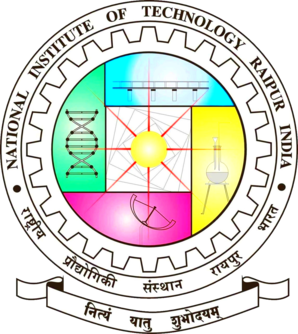
\includegraphics[scale=0.8]{nitlogo.png }
\end{center}
\vspace{1cm}
\begin{center}
   \emph{\large By}\\
\Large{Raj Motwani }\\
\large{Roll No- 21111042}\\
\large{Biomedical 1st Sem}\\
\end{center}
\begin{center}
\newpage
\huge{\underline{The Evolution  of  Cancer Research}}
\end{center}


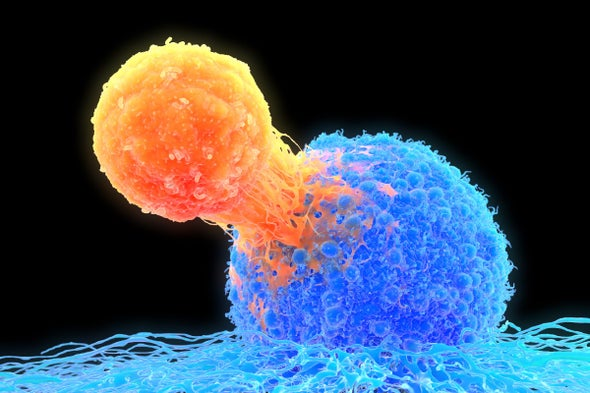
\includegraphics[scale=0.5]{canc.jpg}
%\centering


In 1891, the American cancer researcher William B. Coley injected bacteria into a man’s tumors, and the treatment was successful. More than a century later, scientists are still trying to understand, with precision, why it worked.
“You get cancer all the time, but many mechanisms keep it from becoming an irreversible problem,” says James Smothers, head of GSK’s immuno-oncology and combinations research. Problems occur when those mechanisms fail. Even under powerful attacks from the immune system, cancers routinely fight back. Genetic alterations help the disease evade the immune system, and cancer cells can alter the local immune response.
That devious adaptability can lower responsiveness to therapies, and is why the efficacy of treatments can dwindle over time. To overcome that, scientists are investigating a collection of new therapeutic approaches that release cancer’s hold on the immune system and enhance a patient’s natural immune response, just as injections of bacteria did for Coley’s patient. The results could open a new front in the fight against cancer.\par
\clearpage\par
\section{\underline{Activating the Immune Response:-}}

As a standard of care, traditional chemotherapy is an effective albeit fairly crude approach to eliminating cancer; it targets and kills fast-dividing cells. Immuno-oncology (IO) therapies attack cancer’s survival tactics. For research that earned them a Nobel prize, researchers James Allison and Tasuku Honjo established methods that led to the first widespread IO therapies. They found that cancers can inhibit the body’s T cells, which attack tumor cells. The therapeutics that grew from this work, a category known as checkpoint inhibitors, release a cancer’s hold on T cells, allowing the immune system to once again mount a robust response.
If checkpoint inhibitors release the brakes on T cell responses, Marc Ballas, a medical oncologist, is investigating a treatment approach that steps on the gas. Ballas leads research and development at GSK on agonist antibodies, which could increase the response of T cells to supercharge attacks on a cancer. In Ballas’s view, inhibitors could be combined with an agonist to great effect. “We may be able to dial in and out the impact of each drug on the cancer,” he says. “That way, maybe we could modulate the immune system for just the right degree of response.”
Such flexibility is vital when fighting a disease as mutable as cancer. “Being adaptable is the main advantage of immuno-oncology agents over other cancer therapies,” says Axel Hoos, head of oncology research and development at GSK. “The therapy can change over time — adapting to changes in a tumor, bypassing resistance responses.”
\section{\underline{Enhancing Existing Treatments:-}}
With traditional cancer drugs, delivering therapeutics to the right location at the right moment is an enduring challenge. Biology can be uncooperative. To improve delivery of existing drugs, many researchers are investigating antibody-drug conjugates (ADCs). In essence, ADCs combine a cancer-killing payload and an antibody that binds to a specific cancer cell.
“The antibody is more of a mediator carrying a payload,” said Christoph Rader, who works on antibody-based drugs and new targets for cancer therapy at Scripps Research in Florida. Although ADCs are not technically an IO therapy, since they don’t incite an immune response, Rader says they are, at times, interdependent. “An endogenous T-cell response is very important for ADCs to exert their activity.”
Another approach to improve the efficacy of existing cancer drugs lies in assessing the conditions that surround a cancer. The tumor microenvironment (TME), which is comprised of the cancer and nearby cells, growth factors, transcription factors and so on, has been shown to affect treatments. Frequently, cancers introduce abnormalities into the TME. “These abnormalities fuel tumor growth, metastasis and immune suppression,” says Rakesh Jain, a tumor biologist at Massachusetts General Hospital and Harvard Medical School. He also says that the TME can confer resistance to all kinds of therapies: radiation, chemotherapy, targeted therapy and immunotherapy.
To improve cancer treatments, Jain wants to repair abnormalities in the TME. Using intravital microscopy, he showed that decreases in blood supply to the TME could correlate with increased abnormalities. “By repairing blood flow, any flavor of immunotherapy will work better,” he says.
Jain is particularly interested in drugs that might repair that flow, namely anti-vascular endothelial growth factor (VEGF), which would stop leakage in tumor blood vessels. Though still in early stages, and not applicable to all cancers, his research could point to a broader approach to tumor management. In the past 18 months, the U.S. Food and Drug Administration has approved five combinations of anti-VEGF drugs with checkpoint inhibitors.

\section{\underline{Precision at Scale:-}}

Unlike personalized medicine, a primary focus on IO is the delivery of precise treatments suitable to as many patients as possible. When asked which developing research most excites him, Hoos points to a pathway controlled by the signaling molecule, called the stimulator of interferon genes, or STING.
“Turning on this pathway activates the immune system very broadly,” Hoos says. STING triggers the production of type 1 interferon, which mobilizes a patient’s adaptive immune response to cancer1. That sort of activation triggers a patient’s inherent cancer-fighting response.
Hoos also says that while some therapies need to be injected into a tumor, which limits their breadth, certain research indicates that STING could be administered systemically. “We could perhaps infuse a STING agonist and reach more cancers,” Hoos explains.
While the research on STING is highly sophisticated, with collaborations spanning the globe, today’s scientists and clinical researchers are still, fundamentally pursuing the same work that Coley was more than 120 years ago: looking for ways to turn the immune system against cancer. 
%\subsection{}
%\rule{\textwidth}{1pt}









\enddocument